%---------------------------------------------------------------------
%
%                          contributions.tex
%
%---------------------------------------------------------------------
%
% contributions.tex
% Copyright 2015 Dr. Francisco J. Pulido
%
% This presentation belongs to the PhD titled "New Techniques and Algorithms for Multiobjective and Lexicographic Goal-Based Shortest Path Problems", distributed under the Creative Commons Licence Attribution-NonCommercial-NoDerivs 3.0, available in http://creativecommons.org/licenses/by-nc-nd/3.0/. The complete PhD dissertation is freely accessible from http://www.lcc.uma.es/~francis/

\section{Algorithmic contributions}
%%%%%%%%%%%%%%%%%%%%%%%%%%%%%%%%%%%%%%%%%%%%%%%%%%%%%%%%%%%%%%%%%%%%%%%%%%%%%%%%%%%%%%%%%%%%%%%%%%%%%%%%%
\begin{frame}
\frametitle{Algorithmic contributions}
	\begin{figure}
    	\centering
		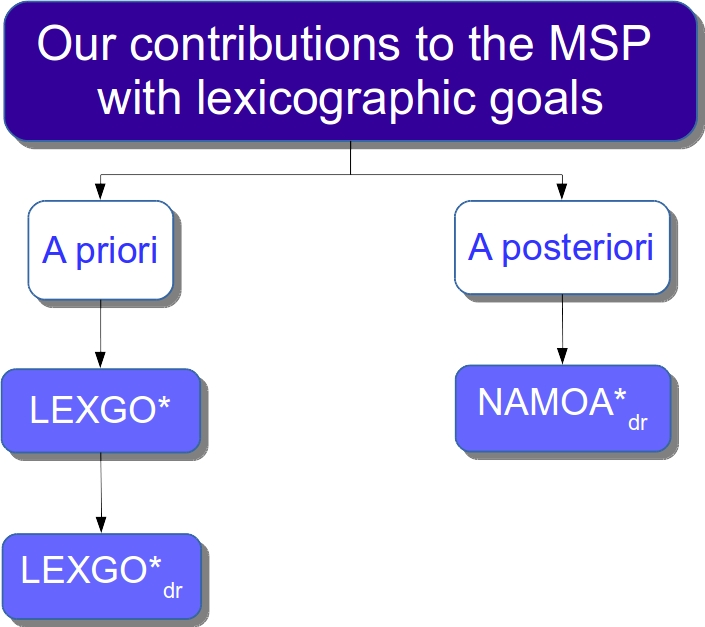
\includegraphics[scale=0.4]{figs/contributions}
	\end{figure}
\note{}
\end{frame}
%%%%%%%%%%%%%%%%%%%%%%%%%%%%%%%%%%%%%%%%%%%%%%%%%%%%%%%%%%%%%%%%%%%%%%%%%%%%%%%%%%%%%%%%%%%%%%%%%%%%%%%%%
\subsection{\texorpdfstring{\lexgo}{\lexgo}}
\begin{frame}
\frametitle{Lexicographic goal preferences}
	\begin{alertblock}{Important!}
		\vspace{1mm}
		Bellman's Principle of Optimality, \textbf{an optimal path is made up of suboptimal paths}, holds for multiobjective search problems, but \textcolor{red}{it does not hold for lexicographic goal preferences!}
		\vspace{1mm}
	\end{alertblock}
\note{Let's remark a fact, the principle of optimality does hold for MSP but it does not hold for lexicographic goals. We need to keep that in mind when we present the new discarding rules for these problems.}
\end{frame}
%%%%%%%%%%%%%%%%%%%%%%%%%%%%%%%%%%%%%%%%%%%%%%%%%%%%%%%%%%%%%%%%%%%%%%%%%%%%%%%%%%%%%%%%%%%%%%%%%%%%%%%%%
\begin{frame}
\frametitle{Lexicographic goal preferences}
	\begin{example}
		\vspace{1mm}
		Two paths $P_1$ and $P_2$ reach some node $n$ with costs $\vec g(P_1) = (\textcolor<2>{red}{8}, \textcolor<2>{red}{8}, \textcolor<3>{red}{12})$ and $\vec g(P_2) = (\textcolor<2>{red}{10}, \textcolor<2>{red}{10}, \textcolor<3>{red}{8})$, respectively. The user goals are defined as follows:
		\vspace{1mm}		
	\end{example}
	\vspace{-4mm}
	\begin{columns}[onlytextwidth, t]
	\column{0.5\linewidth}
	\vspace{4mm}
    \begin{equation*}
     \begin{array}{cll}
     	\textrm{Level 1:} & g_1 \leq 10, & w_1 = 0.5 \\
     					  & g_2 \leq 10, & w_2 = 0.5 \\ 
       	\textrm{Level 2:} & g_3 \leq 10, & w_3 = 1.
     \end{array}
   \end{equation*}	
	\column{0.5\linewidth}
    \begin{figure}
    \centering
    		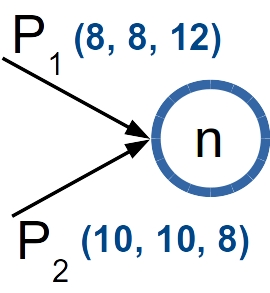
\includegraphics[scale=0.3]{figs/optimality-principle}
  	\end{figure}
	\end{columns}     
   \begin{example}
		\vspace{1mm}	
		The deviation from goals for $P_1$ and $P_2$ is $\vec d(P_1) = (\textcolor<2>{red}{0}, \textcolor<3>{red}{2})$ and $\vec d(P_2) = (\textcolor<2>{red}{0}, \textcolor<3>{red}{0})$, respectively. Thus, \textcolor{ao}{$P_2 \prec_G P_1$}.
		\vspace{1mm}	
	\end{example}
\note{}
\end{frame}
%%%%%%%%%%%%%%%%%%%%%%%%%%%%%%%%%%%%%%%%%%%%%%%%%%%%%%%%%%%%%%%%%%%%%%%%%%%%%%%%%%%%%%%%%%%%%%%%%%%%%%%%%
\begin{frame}
\frametitle{Lexicographic goal preferences}
	\begin{example}
		\vspace{1mm}	
		Let's now consider there is only one additional path $P_3$ to the destination node $t$, such as $\vec g(P_3)) = (2, 2, 2)$. \\
		Therefore, \\ 
		\begin{itemize}
			\item $\vec g(P_1 P_3)) = (\textcolor<2>{red}{10}, \textcolor<2>{red}{10}, \textcolor<3>{red}{14})$ and $\vec g(P_2 P_3)) = (\textcolor<2>{red}{12}, \textcolor<2>{red}{12}, \textcolor<3>{red}{10})$. 
			\item $\vec d(P_1 P_3) = (\textcolor<2>{red}{0},\textcolor<3>{red}{4})$ and $\vec d(P_2 P_3) = (\textcolor<2>{red}{2},\textcolor<3>{red}{0})$. 
			\item Now, \textcolor{ao}{$P_1 P_3 \prec_G P_2 P_3$}
		\end{itemize}
		\textcolor{red}{We have pruned an optimal path!}
		\vspace{1mm}	
	\end{example}
	\begin{figure}
    \centering
    		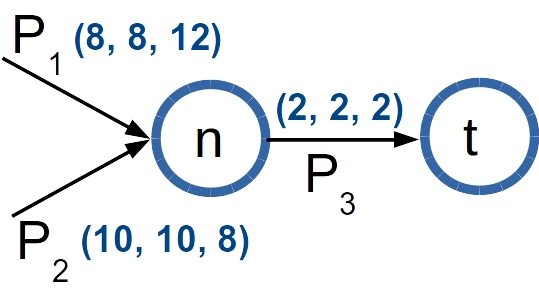
\includegraphics[scale=0.3]{figs/optimality-principle2}
  	\end{figure}
\note{}
\end{frame}
%%%%%%%%%%%%%%%%%%%%%%%%%%%%%%%%%%%%%%%%%%%%%%%%%%%%%%%%%%%%%%%%%%%%%%%%%%%%%%%%%%%%%%%%%%%%%%%%%%%%%%%%%
\begin{frame}
\frametitle{Lexicographic goal preferences}
	\begin{example}
		Let's now assume paths $P_1$ and $P_2$ have costs $\vec g(P_1)$ = (\textcolor<2>{red}{12}, \textcolor<3>{red}{8, 16}) and $\vec g(P_2)$ = (\textcolor<2>{red}{12}, \textcolor<3>{red}{12, 6}), respectively. The user goals are now \emph{different} and defined as follows:
	\end{example}
	\vspace{-6mm}
	\begin{columns}[onlytextwidth, t]
	\column{0.5\linewidth}
	\vspace{3mm}
    \begin{equation*}
     \begin{array}{cll}
     	\textrm{Level 1:} & g_1 \leq 10, & w_1 = 1 \\
     	\textrm{Level 2:} & g_2 \leq 10, & w_2 = 0.5 \\ 
       	 				  & g_3 \leq 10, & w_3 = 0.5. \\
     \end{array}
   \end{equation*}	
	\column{0.5\linewidth}
    \begin{figure}
    \centering
    		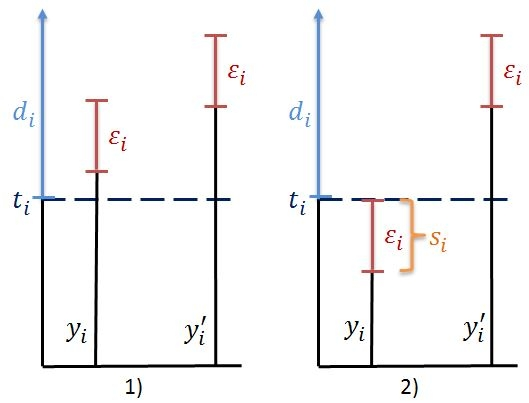
\includegraphics[scale=0.25]{figs/cross-slacks}
  	\end{figure}
	\end{columns}     
   \begin{example}
		The deviation from goals for $P_1$ and $P_2$ is now $\vec d(P_1)$ = (\textcolor<2>{red}{2}, \textcolor<3>{red}{3}) and $\vec d(P_2)$ = (\textcolor<2>{red}{2}, \textcolor<3>{red}{1}), respectively. $P_2 \prec_G P_1$, but, can $P_1$ be \textcolor{red}{safely} pruned?
	\end{example}
\note{}
\end{frame}
%%%%%%%%%%%%%%%%%%%%%%%%%%%%%%%%%%%%%%%%%%%%%%%%%%%%%%%%%%%%%%%%%%%%%%%%%%%%%%%%%%%%%%%%%%%%%%%%%%%%%%%%%
\begin{frame}
\frametitle{Discarding labels by deviation}
	Deviation-based pruning ($\prec_P$)
	\vspace{5mm}
	\begin{columns}[onlytextwidth, t]
	\column{0.35\linewidth}
	\textit{Slack variable} \\
	\vspace{1mm}	
	\Ovalbox{$s_k = \max(0, t_k - y_k)$}
	\column{0.6\linewidth}
	\textit{Cross slacks} \\
	\vspace{1mm}	
	\Ovalbox{$\delta_j(\vec{y}, \vec{y'}) = \sum_{k\in I_j} w_k \times \max(0, s'_k - s_k)$}
	\end{columns}
	\vspace{3mm}
	\begin{example}
		\vspace{1mm}
		Given $\vec g(P_1)$ = (12, \textcolor<2>{red}{8}, 16) and \ $\vec g(P_2)$ = (12, 12, \textcolor<3>{red}{6}),\\
		where $\vec d(P_1)$ = (2, \textcolor<5>{red}{3}) and \ $\vec d(P_2)$ = (2, \textcolor<5>{red}{1}):
		\begin{itemize}
			\item \textcolor<2>{red}{$s_2(P_1) = (10 - 8) \times 0.5 = \textcolor<4>{red}{1}$.} 
			\item \textcolor<3>{red}{$s_3(P_2) = (10 - 6) \times 0.5 = \textcolor<4>{red}{2}.$} 
			\item \textcolor<4>{red}{$\delta_2(P_1, P_2)= 2 - 1 = \textcolor<6>{red}{1}$,} 
		\end{itemize}
		\textcolor<5>{red}{Finally, $d_2(P_2) - d_2(P_1) = 3 - 1 = 2$} $>$ \textcolor<6>{red}{1}.
		\vspace{1mm}		
	\end{example}
\note{}
\end{frame}
%%%%%%%%%%%%%%%%%%%%%%%%%%%%%%%%%%%%%%%%%%%%%%%%%%%%%%%%%%%%%%%%%%%%%%%%%%%%%%%%%%%%%%%%%%%%%%%%%%%%%%%%%
\begin{frame}
\frametitle{Discarding labels by deviation}
Deviation-based pruning ($\prec_P$) \\
	\vspace{3mm}
     $ \vec{y} \prec_{P} \vec{y'} \ \ \Leftrightarrow \ \ $ \textcolor<2>{red}{$\forall i < j
      \ \ (d_i(\vec{y}) = d_i(\vec{y'}) \ \quad \land \quad \delta_i(\vec{y}, \vec{y'}) = 0))$} $\quad \land$ \\
     \vspace{3mm}
     \qquad \qquad \qquad \qquad \textcolor<3>{red}{$\exists j \ (d_j(\vec{y}) < d_j(\vec{y'}) \quad \land \quad \delta_j(\vec{y}, \vec {y'}) < d_j(\vec{y'}) - d_j(\vec{y})$} \\
	\vspace{5mm}
	Deviation-based filtering
	\vspace{3mm}
	\begin{equation*}
     \vec{d_B} \prec_{L} \vec{d}
    \end{equation*}
\end{frame}
%%%%%%%%%%%%%%%%%%%%%%%%%%%%%%%%%%%%%%%%%%%%%%%%%%%%%%%%%%%%%%%%%%%%%%%%%%%%%%%%%%%%%%%%%%%%%%%%%%%%%%%%%
\begin{frame}
\frametitle{\lexgo}	
	\begin{framed}
		\textcolor{ao}{In addition to the pruning and filtering rules of \namoa}, 
		\lexgo \ also uses its own rules to prune and filter paths by deviation.
	\end{framed}
\note{}
\end{frame}	
%%%%%%%%%%%%%%%%%%%%%%%%%%%%%%%%%%%%%%%%%%%%%%%%%%%%%%%%%%%%%%%%%%%%%%%%%%%%%%%%%%%%%%%%%%%%%%%%%%%%%%%%%
\begin{frame}
\frametitle{\lexgo}
	\begin{alertblock}{\lexgo \ shares \namoa \ formal properties}
		\begin{itemize}
		\vspace{2mm}
		\item The \textcolor{red}{new} deviation-based pruning and filtering rules \textcolor{red}{do not discard} goal-optimal solutions.
		\vspace{2mm}
 		\item \lexgo \ \textcolor{red}{always} returns the set of all goal-optimal solutions.
		\vspace{2mm}
 		\item \lexgo \ expands a \textcolor{red}{subset} of the labels expanded by \namoa.
 		\vspace{2mm}
		\end{itemize}
	\end{alertblock}
\note{}
\end{frame}
%%%%%%%%%%%%%%%%%%%%%%%%%%%%%%%%%%%%%%%%%%%%%%%%%%%%%%%%%%%%%%%%%%%%%%%%%%%%%%%%%%%%%%%%%%%%%%%%%%%%%%%%%
\subsection{T-discarding}
\begin{frame} 
\frametitle{T-discarding}
	\begin{block}{Limiting factor in MSP}
	\vspace{1mm}
		\textcolor{ao}{Runtime}, rather than memory, is the \textcolor{ao}{limiting factor} in multicriteria search algorithms performance, as well as in the size of problems that can be practically solved.
	\vspace{1mm}
	\end{block}
	\vspace{8mm}
	\begin{block}{Limiting factor in MSP (II)}
	\vspace{1mm}
		The \textcolor{ao}{majority} of the algorithm \textcolor{ao}{runtime} can be attributed to dominance checks against $G_{op}, G_{cl}$ and COSTS to discard dominated paths. 
	\vspace{1mm}
	\end{block}
\note{T-discarding arose due to time rather memory is nowadays the limiting factor in multicriteria search algorithms performance. This runtime can be mostly attributed to dominance checks to discard paths. In this manner, if we speed up these checks, we will speed up the algorithms.}
\end{frame}
%%%%%%%%%%%%%%%%%%%%%%%%%%%%%%%%%%%%%%%%%%%%%%%%%%%%%%%%%%%%%%%%%%%%%%%%%%%%%%%%%%%%%%%%%%%%%%%%%%%%%%%%%
\begin{frame}
\frametitle{T-discarding}
	Let's suppose a typical scenario where a new path with cost $\vec v$ reaches some node $n$. This node \textcolor{ao}{has already three closed paths} with costs $(\vec x, \vec y, \vec z)$. Let's now \textcolor{ao}{check if $\vec v$ is dominated} by any vector in $G_{cl}(n)$:
	\vspace{5mm}
	\begin{columns}%[onlytextwidth, t]
	\column{0.5\linewidth}
	\begin{example}
	\vspace{1mm}
	\begin{itemize}
		\item $\vec x \prec \vec v$ ? \ $\rightarrow$ \ $x_1 \leq v_1$, $x_2 \leq v_2$ ...
		\item $\vec y \prec \vec v$ ? \ $\rightarrow$ \ $y_1 \leq v_1$, $y_2 \leq v_2$ ...
		\item $\vec z \prec \vec v$ ? \ $\rightarrow$ \ $z_1 \leq v_1$, $z_2 \leq v_2$ ...
	\end{itemize}
	Worst-case scenario: \\ 
	\begin{itemize}
		\item 3 vector comparisons
		\item 9 scalar comparisons
	\end{itemize}
	\end{example}
	\column{0.5\linewidth}
	\begin{figure}
    	\centering
		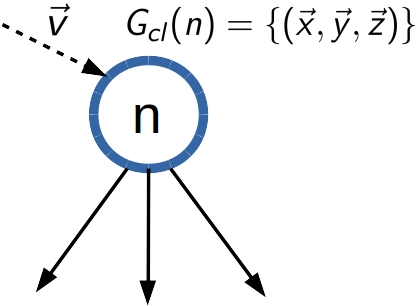
\includegraphics[scale=0.45]{figs/t-discarding}
	\end{figure}
	\end{columns}
\note{}
\end{frame}	
%%%%%%%%%%%%%%%%%%%%%%%%%%%%%%%%%%%%%%%%%%%%%%%%%%%%%%%%%%%%%%%%%%%%%%%%%%%%%%%%%%%%%%%%%%%%%%%%%%%%%%%%%
\begin{frame} 
\frametitle{T-discarding}
	\begin{block}{Definition}
		\vspace{1mm}
		T-discarding (\emph{truncated discarding}) is a dimensionality reduction technique to \textcolor{ao}{speed up dominance checks}.
		\vspace{1mm}
	\end{block}
\note{This is the definition of our proposal, called t-discarding, or truncated distarding. This proposal is based on a dimensionality reduction technique to speed up dominance checks.}
\end{frame}	
%%%%%%%%%%%%%%%%%%%%%%%%%%%%%%%%%%%%%%%%%%%%%%%%%%%%%%%%%%%%%%%%%%%%%%%%%%%%%%%%%%%%%%%%%%%%%%%%%%%%%%%%%
\begin{frame}[t]
\frametitle{T-discarding}
	\begin{block}{Assumptions}
		\vspace{1mm}
		To apply t-discarding an algorithm must have:
		\begin{itemize}
			\item Lexicographic order as label selection policy.
			\item One consistent heuristic function as lower bound. 
		\end{itemize}
		\vspace{1mm}
	\end{block}
	\only<2-3>{
	\begin{example}
	When \textcolor{ao}{lexicographic order} is used to select open paths:
	\vspace{-2mm}
	\begin{columns}[onlytextwidth, t]
	\column{0.5\linewidth}
		\begin{itemize}
			\item<2> $\rightarrow$ (3, 5, 7)
			\item<2> $\rightarrow$ (4, 6, 4)
			\item<2> $\rightarrow$ (4, 6, 7)
			\item<2> $\rightarrow$ (6, 2, 4)
		\end{itemize}
	\column{0.5\linewidth}
		\begin{itemize}
			\item<3> $\rightarrow$ (3, -, -)
			\item<3> $\rightarrow$ (4, -, -)
			\item<3> $\rightarrow$ (4, -, -)
			\item<3> $\rightarrow$ (6, -, -)
		\end{itemize}	
	\end{columns}	
	\end{example}
	}
	\only<4>{
	\vspace{5mm}	
	\begin{alertblock}{Property}
		Assuming the last selected open path had cost $\vec c = c_1, c_2, ..., c_q$, the next path selected to be open with cost $\vec{c'} = c'_1, c'_2, ..., c'_q$ \textcolor{red}{must have} $c'_1 \geq c_1$ !
	\end{alertblock}
	}
\note{Do we have some assumptions before applying this technique? Yes, two assumptions, the first one is to use a lexicographic order as label selection policy, and the second one, is to use a consistent heuristic function as lower bound.
We can depict here the main idea. This is the representation of 3 vectors x, y, and z. What happens if we ignore the first objective and we represent the three truncated vectors only according to the second and third objectives? We observe that the truncated vector x dominates the other two... 
}
\end{frame}
%%%%%%%%%%%%%%%%%%%%%%%%%%%%%%%%%%%%%%%%%%%%%%%%%%%%%%%%%%%%%%%%%%%%%%%%%%%%%%%%%%%%%%%%%%%%%%%%%%%%%%%%%
\begin{frame}
\frametitle{T-discarding}
	Let's suppose a typical scenario where a new path with cost $\vec v$ reaches some node $n$. This node \textcolor{ao}{has already three closed paths} with costs $(\vec x, \vec y, \vec z)$. Let's now \textcolor{ao}{check if $\vec v$ is dominated} by any vector in $G_{cl}(n)$:
	\vspace{5mm}
	\begin{columns}%[onlytextwidth, t]
	\column{0.5\linewidth}
	\begin{example}
	\vspace{1mm}
	\begin{itemize}
		\item $\vec x \prec \vec v$ ? \ $\rightarrow$ \ $x_1 \leq v_1$, $x_2 \leq v_2$ ...
		\item $\vec y \prec \vec v$ ? \ $\rightarrow$ \ $y_1 \leq v_1$, $y_2 \leq v_2$ ...
		\item $\vec z \prec \vec v$ ? \ $\rightarrow$ \ $z_1 \leq v_1$, $z_2 \leq v_2$ ...
	\end{itemize}
	Worst-case scenario: \\ 
	\begin{itemize}
		\item 3 vector comparisons
		\item 9 scalar comparisons
	\end{itemize}
	\end{example}
	\column{0.5\linewidth}
	\begin{figure}
    	\centering
		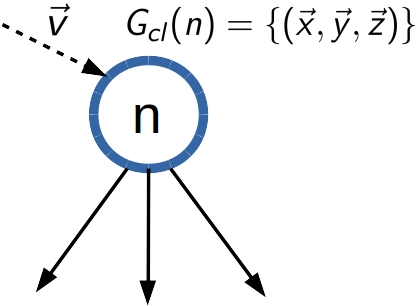
\includegraphics[scale=0.45]{figs/t-discarding}
	\end{figure}
	\end{columns}
\note{}
\end{frame}	
%%%%%%%%%%%%%%%%%%%%%%%%%%%%%%%%%%%%%%%%%%%%%%%%%%%%%%%%%%%%%%%%%%%%%%%%%%%%%%%%%%%%%%%%%%%%%%%%%%%%%%%%%
\begin{frame}
\frametitle{T-discarding}
	\begin{figure}
    	\centering
		\includegraphics<1>[scale=0.4]{figs/t-discarding1}
		\includegraphics<2>[scale=0.4]{figs/t-discarding2}
		\includegraphics<3>[scale=0.4]{figs/t-discarding3}
	\end{figure}
\note{}
\end{frame}
%%%%%%%%%%%%%%%%%%%%%%%%%%%%%%%%%%%%%%%%%%%%%%%%%%%%%%%%%%%%%%%%%%%%%%%%%%%%%%%%%%%%%%%%%%%%%%%%%%%%%%%%%
\begin{frame}
\frametitle{T-discarding}
	Let's suppose a typical scenario where a new path with cost $\vec v$ reaches some node $n$. This node \textcolor{ao}{has already three closed paths} with costs $(\vec x, \vec y, \vec z)$. Let's now \textcolor{ao}{check if $\vec v$ is dominated} by any vector in $G_{cl}(n)$:
	\vspace{5mm}
	\begin{columns}%[onlytextwidth, t]
	\column{0.5\linewidth}
	\begin{example}
	\vspace{1mm}
	\begin{itemize}
		\item $\vec x \prec \vec v$ ? \ $\rightarrow$ \ $x_1 \leq v_1$, $x_2 \leq v_2$ ...
		\item $\vec y \prec \vec v$ ? \ $\rightarrow$ \ $y_1 \leq v_1$, $y_2 \leq v_2$ ...
		\item $\vec z \prec \vec v$ ? \ $\rightarrow$ \ $z_1 \leq v_1$, $z_2 \leq v_2$ ...
	\end{itemize}
	Worst-case scenario: \\ 
	\begin{itemize}
		\item 3 vector comparisons
		\item 9 scalar comparisons
	\end{itemize}
	\end{example}
	\column{0.5\linewidth}
	\begin{figure}
    	\centering
		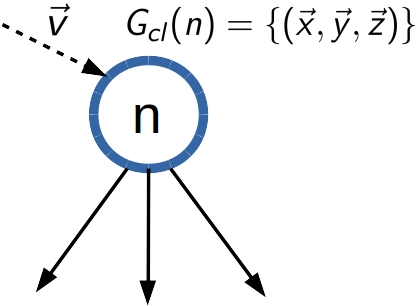
\includegraphics[scale=0.45]{figs/t-discarding}
	\end{figure}
	\end{columns}
\note{}
\end{frame}	
%%%%%%%%%%%%%%%%%%%%%%%%%%%%%%%%%%%%%%%%%%%%%%%%%%%%%%%%%%%%%%%%%%%%%%%%%%%%%%%%%%%%%%%%%%%%%%%%%%%%%%%%%
\begin{frame}
\frametitle{T-discarding}
	Is a vector \textcolor{ao}{$\vec v$ dominated} by any vector in the previous set $(\vec x, \vec y, \vec z)$? 
	\vspace{8mm}
	\begin{block}{Standard discarding}
	\vspace{1mm}
	$\vec v$ \textcolor{ao}{must be compared to} $(\vec x, \vec y, \vec z)$ to check if it is dominated.
	\vspace{1mm} 
	\end{block}
	\vspace{3mm}
	\begin{block}{T-discarding}
	\vspace{1mm}
	 The truncated vector $t(\vec v)$ \textcolor{ao}{must be compared only to} $t(\vec x)$ to check if it is dominated. 
	 \vspace{1mm}
	\end{block}			
\note{}
\end{frame}
%%%%%%%%%%%%%%%%%%%%%%%%%%%%%%%%%%%%%%%%%%%%%%%%%%%%%%%%%%%%%%%%%%%%%%%%%%%%%%%%%%%%%%%%%%%%%%%%%%%%%%%%%
\begin{frame}
\frametitle{T-discarding}
\begin{block}{Benefits of t-discarding}
	\vspace{1mm}
		\begin{itemize}
			\item Dominance checks can be done with vectors \textcolor{ao}{reduced in one dimension}.
			\vspace{1mm}
			\item \textcolor{ao}{The size of sets} $T(G_{cl}(n))$ and $T(COSTS)$ \textcolor{ao}{is also reduced}.
		\end{itemize}
	\vspace{1mm}
	\end{block}
	\vspace{2mm}
	\begin{alertblock}{Important!}
		\vspace{1mm}
		T-discarding only implies checking dominance against different sets:
		\begin{itemize}
			\item \textcolor{red}{Very simple implementation.}
			\vspace{1mm}
			\item Any label discarded by standard pruning \textcolor{red}{$\Longleftrightarrow$} is discarded by t-discarding.
			\vspace{1mm}
			\item \textcolor{red}{Does not affect any formal property} of the algorithm.
		\end{itemize}			
	\end{alertblock}
\note{}
\end{frame}
%%%%%%%%%%%%%%%%%%%%%%%%%%%%%%%%%%%%%%%%%%%%%%%%%%%%%%%%%%%%%%%%%%%%%%%%%%%%%%%%%%%%%%%%%%%%%%%%%%%%%%%%%
\subsection{\texorpdfstring{\namoadr}{\namoadr}}
\begin{frame} 
\frametitle{\namoadr}
	The applicability of t-discarding to \namoa \ is \textcolor{ao}{full} and straightforward:
	\vspace{4mm}
	\begin{framed}
		Cl-pruning and filtering are now performed against: 
    		\vspace{3mm}
		\begin{itemize}
			\item $T(G_{cl}(n))$
			\vspace{3mm}
			\item T(COSTS)
		\end{itemize} 	 
	\end{framed} 
\note{}
\end{frame}
%%%%%%%%%%%%%%%%%%%%%%%%%%%%%%%%%%%%%%%%%%%%%%%%%%%%%%%%%%%%%%%%%%%%%%%%%%%%%%%%%%%%%%%%%%%%%%%%%%%%%%%%%
\subsection{\texorpdfstring{\lexgodr}{\lexgodr}}
\begin{frame} 
\frametitle{\lexgodr}
	The applicability of t-discarding to \lexgo \ is \textcolor{red}{partial}:
	\vspace{4mm}
	\begin{framed}
		Cl-pruning and filtering are now performed against: 
    		\vspace{3mm}
		\begin{itemize}
			\item $T(G_{cl}(n))$
			\vspace{3mm}
			\item T(COSTS)
		\end{itemize} 
		\vspace{3mm}	
		but \textcolor{red}{only when $\vec d = 0$}. 
	\end{framed} 
\note{}
\end{frame}
%%%%%%%%%%%%%%%%%%%%%%%%%%%%%%%%%%%%%%%%%%%%%%%%%%%%%%%%%%%%%%%%%%%%%%%%%%%%%%%%%%%%%%%%%%%%%%%%%%%%%%%%%
\begin{frame}
\frametitle{Summary}
	\begin{table}
	\centering
	\scalebox{1}{
	\begin{tabular}{|lllll|}
	\hline \noalign{\smallskip}
	& \namoa & \lexgo & \namoadr & \lexgodr \\
	\noalign{\smallskip} \hline \noalign{\smallskip}
	Op-pruning & $G_{op}(n)$ & $G_{op}(n)$ & $G_{op}(n)$ & $G_{op}(n)$ \\
	\noalign{\smallskip} \hline \noalign{\smallskip}
	Cl-pruning & $G_{cl}(n)$ & $G_{cl}(n)$ & $T(G_{cl}(n))$ & $T(G_{cl}(n))$* \\
	\noalign{\smallskip} \hline \noalign{\smallskip}
	Filtering & COSTS & COSTS & T(COSTS) & T(COSTS)* \\
	\noalign{\smallskip} \hline \noalign{\smallskip}
	\end{tabular}
	}
	\end{table}
\note{}
\end{frame}
